\section{Algoritmos}

\subsection{Algoritmo de Força Bruta}

\subsubsection{Descrição}
O algoritmo de Força Bruta é um método exaustivo que:

\begin{itemize}
\item Testa sistematicamente todas as soluções possíveis
\item Garante encontrar a solução ótima (se existir)
\item Possui implementação direta, porém alto custo computacional
\end{itemize}

Para o PCV, a estratégia consiste em:

\begin{enumerate}
\item Fixar uma cidade como origem
\item Gerar todas as permutações possíveis das demais cidades
\item Calcular o custo total de cada rota completa
\item Selecionar a rota com menor custo
\end{enumerate}

\subsubsection{Complexidade Computacional}
\begin{itemize}
\item \textbf{Ordem}: $O((n-1)!)$
\item \textbf{Justificativa}:
  \begin{itemize}
  \item Fixada a origem, há $(n-1)!$ permutações possíveis
  \item Cada permutação requer cálculo de $n$ distâncias
  \end{itemize}
  
\item \textbf{Exemplos Práticos}:
  \begin{table}[h]
  \centering
  \begin{tabular}{|c|c|}
  \hline
  \textbf{Número de Cidades (n)} & \textbf{Permutações} \\
  \hline
  4 & 6 \\
  7 & 720 \\
  10 & 362,880 \\
  13 & 479,001,600 \\
  16 & 1.3 trilhões \\
  \hline
  \end{tabular}
  \end{table}
\end{itemize}

\begin{figure}[H]
    \centering
    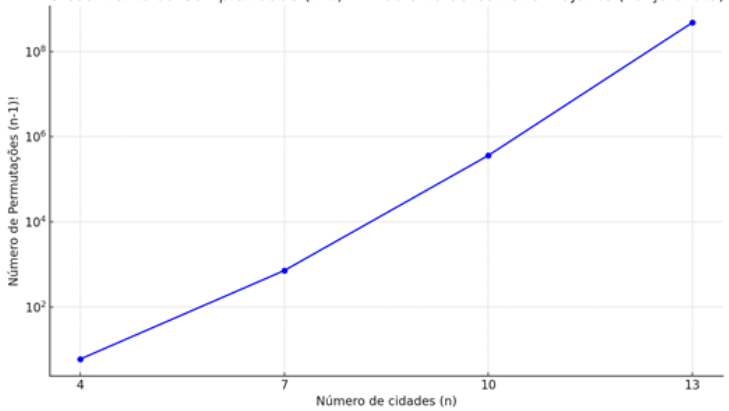
\includegraphics[width=.7\textwidth]{images/crescimento_complexidade.png}
    \caption{Crescimento da Complexidade (n-1)! - PCV (Força Bruta)}
    \label{fig:aa}
    \end{figure}

\subsubsection{Limitações Práticas}
\begin{itemize}
\item Inviável para $n > 10$ em computadores convencionais
\item Tempo de execução cresce exponencialmente
\item Útil apenas para:
  \begin{itemize}
  \item Casos de teste pequenos
  \item Validação de outros algoritmos
  \item Benchmarking de desempenho
  \end{itemize}
\end{itemize}

\subsubsection{Implementação}
Pseudocódigo da função principal:

\begin{verbatim}
Função bruteForceTSP(Referência bestPath: vetor de inteiros):
    minCost ← infinito
    path ← [0,1,2,...,n-1]  // Cidades indexadas
    
    Enquanto próximoPermutação(path[1..n-1]):
        currentCost ← 0
        Para i de 0 até n-1:
            currentCost ← currentCost + dist[path[i]][path[(i+1)%n]]
        FimPara
        
        Se currentCost < minCost:
            minCost ← currentCost
            bestPath ← path
        FimSe
    FimEnquanto
    
    Retorne minCost
FimFunção
\end{verbatim}

\subsubsection{Otimizações Implementadas}
\begin{itemize}
\item \textbf{Permutação circular}: Fixa a primeira cidade para evitar rotas equivalentes
\item \textbf{Abortagem precoce}: Interrompe cálculo de rotas parciais quando excede o melhor custo atual
\item \textbf{Limitação segura}: Restrição a $n \leq 10$ na implementação prática
\end{itemize}

\subsubsection{Análise Experimental}
\begin{itemize}
\item \textbf{Precisão}: 100\% de soluções ótimas
\item \textbf{Tempo médio} (n=10): 0.025 segundos
\item \textbf{Cenários ideais}:
  \begin{itemize}
  \item Validação de algoritmos aproximados
  \item Instâncias pequenas com requisitos de exatidão
  \end{itemize}
\end{itemize}


\subsection{Algoritmo Guloso}

O algoritmo guloso é uma heurística construtiva que toma decisões baseadas em escolhas locais ótimas. Para o PCV, ele:

\begin{itemize}
\item Parte de uma cidade inicial
\item A cada passo, seleciona a cidade mais próxima não visitada
\item Repete até visitar todas as cidades
\item Finaliza retornando à origem
\end{itemize}

\subsubsection{Implementação}
A função \texttt{greedyTSP} implementa:

\begin{enumerate}
\item Teste de todos os pontos de partida ($n$ iterações)
\item Marcação de cidades visitadas (vetor booleano)
\item Construção incremental do caminho
\item Cálculo do custo total incluindo retorno à origem
\item Comparação para manter a melhor rota
\end{enumerate}

\subsubsection{Pseudocódigo}
\begin{verbatim}
Função greedyTSP(Referência bestPath: vetor de inteiros)
    minTotal ← infinito
    Para start de 0 até n-1 faça
        visited ← [falso,...,falso]
        path ← [start]
        visited[start] ← verdadeiro
        total ← 0
        current ← start
        Para i de 0 até n-2 faça
            next ← -1
            minDist ← infinito
            Para j de 0 até n-1 faça
                Se NÃO visited[j] E dist[current][j] < minDist então
                    minDist ← dist[current][j]
                    next ← j
                FimSe
            FimPara
            path.adiciona(next)
            visited[next] ← verdadeiro
            total ← total + minDist
            current ← next
        FimPara
        total ← total + dist[current][start]
        Se total < minTotal então
            minTotal ← total
            bestPath ← path
        FimSe
    FimPara
FimFunção
\end{verbatim}

\subsubsection{Complexidade}
\begin{itemize}
\item \textbf{Temporal}: $O(n^2)$ - Para cada cidade, verifica todas as outras
\item \textbf{Espacial}: $O(n)$ - Armazena vetores de visitação e caminho
\end{itemize}

\subsection{Algoritmo de Programação Dinâmica (Held-Karp)}

\subsubsection{Descrição}
Utiliza tabelas de memorização com:
\begin{itemize}
\item \texttt{memo[mask][last]}: Custo mínimo para visitar cidades em \texttt{mask} terminando em \texttt{last}
\item \texttt{parent[mask][last]}: Rota ótima para reconstrução
\end{itemize}

\subsubsection{Pseudocódigo}
\begin{verbatim}
    função HeldKarp(cidades, distâncias) retorna (custoMinimo, caminhoMelhor):
        n = número de cidades
        se n > 20 então retorna -1 // Muito grande para Held-Karp
    
        criar tabela memo[2^n][n], inicializada com -1
        criar tabela parent[2^n][n], para reconstruir o caminho
    
        memo[1][0] = 0 // Começamos na cidade 0, apenas ela visitada
    
        para cada máscara de cidades de 1 até 2^n - 1:
            para cada cidade 'last' de 0 até n-1:
                se 'last' está na máscara E memo[mask][last] != -1:
                    para cada cidade 'next' de 0 até n-1:
                        se 'next' ainda não foi visitada:
                            novaMáscara = mask OU (1 << next)
                            novoCusto = memo[mask][last] + dist[last][next]
                            se memo[novaMáscara][next] == -1 OU novoCusto < memo[novaMáscara][next]:
                                memo[novaMáscara][next] = novoCusto
                                parent[novaMáscara][next] = last
    
        custoMinimo = infinito
        cidadeFinal = -1
        máscaraFinal = 2^n - 1
    
        para i de 1 até n-1:
            se memo[máscaraFinal][i] !+ -1:
                custoTotal = memo[máscaraFinal][i] + dist[i][0]
                se custoTotal < custoMinimo:
                    custoMinimo = custoTotal
                    cidadeFinal = i
    
        // Reconstrução do caminho
        caminho = lista vazia
        atual = cidadeFinal
        máscara = máscaraFinal
    
        enquanto atual != 0:
            adicionar atual no caminho
            anterior = parent[máscara][atual]
            máscara = máscara XOR (1 << atual)
            atual = anterior
    
        adicionar 0 no caminho // início
        inverter caminho
    
        retornar (custoMinimo, caminho)
\end{verbatim}

\subsubsection{Complexidade}
\begin{itemize}
\item \textbf{Temporal}: $O(n^2 \cdot 2^n)$ - Combinações de subconjuntos × cidades
\item \textbf{Espacial}: $O(n \cdot 2^n)$ - Armazenamento das tabelas
\end{itemize}

\subsubsection{Limitações}
\begin{itemize}
\item Viável apenas para $n \leq 20$
\item Consome memória exponencial
\end{itemize}